\documentclass[a4paper, 12pt]{article}

% packages
\usepackage{amssymb}
\usepackage[fleqn]{mathtools}
\usepackage{tikz}
\usepackage{enumerate}
\usepackage{bussproofs}
\usepackage{xcolor}
\usepackage[margin=1.3cm]{geometry}
\usepackage{logicproof}
\usepackage{diagbox}
\usepackage{listings}
\usepackage{graphicx}
\usepackage{lstautogobble}
\usepackage{hyperref}
\usepackage{multirow}
\usepackage{tipa}
\usepackage{pgfplots}
\usepackage{adjustbox}
\usepackage{ifthen}

% tikz libraries
\usetikzlibrary{
    decorations.pathreplacing,
    arrows,
    shapes,
    shapes.gates.logic.US,
    circuits.logic.US,
    calc,
    automata,
    positioning,
    intersections
}

\pgfplotsset{compat=1.16}

\pgfmathdeclarefunction{gauss}{2}{%
  \pgfmathparse{1/(#2*sqrt(2*pi))*exp(-((x-#1)^2)/(2*#2^2))}%
}

\allowdisplaybreaks % allow environments to break
\setlength\parindent{0pt} % no indent

% shorthand for verbatim
% this clashes with logicproof, so maybe fix this at some point?
\catcode`~=\active
\def~#1~{\texttt{#1}}

% code listing
\lstdefinestyle{main}{
    numberstyle=\tiny,
    breaklines=true,
    showspaces=false,
    showstringspaces=false,
    tabsize=2,
    numbers=left,
    basicstyle=\ttfamily,
    columns=fixed,
    fontadjust=true,
    basewidth=0.5em,
    autogobble,
    xleftmargin=3.0ex,
    mathescape=true
}
\newcommand{\dollar}{\mbox{\textdollar}} %
\lstset{style=main}

% augmented matrix
\makeatletter
\renewcommand*\env@matrix[1][*\c@MaxMatrixCols c]{%
\hskip -\arraycolsep
\let\@ifnextchar\new@ifnextchar
\array{#1}}
\makeatother

% ceiling / floor
\DeclarePairedDelimiter{\ceil}{\lceil}{\rceil}
\DeclarePairedDelimiter{\floor}{\lfloor}{\rfloor}

% custom commands
\newcommand{\indefint}[2]{\int #1 \, \mathrm{d}#2}
\newcommand{\defint}[4]{\int_{#1}^{#2} #3 \, \mathrm{d}#4}
\newcommand{\pdif}[2]{\frac{\partial #1}{\partial #2}}
\newcommand{\dif}[2]{\frac{\mathrm{d}#1}{\mathrm{d}#2}}
\newcommand{\limit}[2]{\raisebox{0.5ex}{\scalebox{0.8}{$\displaystyle{\lim_{#1 \to #2}}$}}}
\newcommand{\limitsup}[2]{\raisebox{0.5ex}{\scalebox{0.8}{$\displaystyle{\limsup_{#1 \to #2}}$}}}
\newcommand{\summation}[2]{\sum\limits_{#1}^{#2}}
\newcommand{\product}[2]{\prod\limits_{#1}^{#2}}
\newcommand{\intbracket}[3]{\left[#3\right]_{#1}^{#2}}
\newcommand{\laplace}{\mathcal{L}}
\newcommand{\fourier}{\mathcal{F}}
\newcommand{\mat}[1]{\boldsymbol{#1}}
\renewcommand{\vec}[1]{\boldsymbol{#1}}
\newcommand{\rowt}[1]{\begin{bmatrix}
    #1
\end{bmatrix}^\top}
\DeclareMathOperator*{\argmax}{argmax}
\DeclareMathOperator*{\argmin}{argmin}

\newcommand{\lto}[0]{\leadsto\ }

\newcommand{\ulsmash}[1]{\underline{\smash{#1}}}

\newcommand{\powerset}[0]{\wp}
\renewcommand{\emptyset}[0]{\varnothing}

\makeatletter
\newsavebox{\@brx}
\newcommand{\llangle}[1][]{\savebox{\@brx}{\(\m@th{#1\langle}\)}%
  \mathopen{\copy\@brx\kern-0.5\wd\@brx\usebox{\@brx}}}
\newcommand{\rrangle}[1][]{\savebox{\@brx}{\(\m@th{#1\rangle}\)}%
  \mathclose{\copy\@brx\kern-0.5\wd\@brx\usebox{\@brx}}}
\makeatother
\newcommand{\lla}{\llangle}
\newcommand{\rra}{\rrangle}
\newcommand{\la}{\langle}
\newcommand{\ra}{\rangle}
\newcommand{\crnr}[1]{\text{\textopencorner} #1 \text{\textcorner}}
\newcommand{\bnfsep}[0]{\ |\ }
\newcommand{\concsep}[0]{\ ||\ }

\newcommand{\axiom}[1]{\AxiomC{#1}}
\newcommand{\unary}[1]{\UnaryInfC{#1}}
\newcommand{\binary}[1]{\BinaryInfC{#1}}
\newcommand{\trinary}[1]{\TrinaryInfC{#1}}
\newcommand{\quaternary}[1]{\QuaternaryInfC{#1}}
\newcommand{\quinary}[1]{\QuinaryInfC{#1}}
\newcommand{\dproof}[0]{\DisplayProof}
\newcommand{\llabel}[1]{\LeftLabel{\scriptsize #1}}
\newcommand{\rlabel}[1]{\RightLabel{\scriptsize #1}}

\newcommand{\ttbs}{\char`\\}
\newcommand{\lrbt}[0]{\ \bullet\ }

% colours
\newcommand{\violet}[1]{\textcolor{violet}{#1}}
\newcommand{\blue}[1]{\textcolor{blue}{#1}}
\newcommand{\red}[1]{\textcolor{red}{#1}}
\newcommand{\teal}[1]{\textcolor{teal}{#1}}

% reasoning proofs
\usepackage{ltablex}
\usepackage{environ}
\keepXColumns
\NewEnviron{reasoning}{
    \begin{tabularx}{\textwidth}{rlX}
        \BODY
    \end{tabularx}
}
\newcommand{\proofline}[3]{$(#1)$ & $#2$ & \hfill #3 \smallskip \\}
\newcommand{\proofarbitrary}[1]{& take arbitrary $#1$ \smallskip \\}
\newcommand{\prooftext}[1]{\multicolumn{3}{l}{#1} \smallskip \\}
\newcommand{\proofmath}[3]{$#1$ & = $#2$ & \hfill #3 \smallskip \\}
\newcommand{\prooftherefore}[1]{& $\therefore #1$ \smallskip \\}
\newcommand{\proofbc}[0]{\prooftext{\textbf{Base Case}}}
\newcommand{\proofis}[0]{\prooftext{\textbf{Inductive Step}}}

% ER diagrams
\newcommand{\nattribute}[4]{
    \node[draw, state, inner sep=0cm, minimum size=0.2cm, label=#3:{#4}] (#1) at (#2) {};
}
\newcommand{\mattribute}[4]{
    \node[draw, state, accepting, inner sep=0cm, minimum size=0.2cm, label=#3:{#4}] (#1) at (#2) {};
}
\newcommand{\dattribute}[4]{
    \node[draw, state, dashed, inner sep=0cm, minimum size=0.2cm, label=#3:{#4}] (#1) at (#2) {};
}
\newcommand{\entity}[3]{
    \node[] (#1-c) at (#2) {#3};
    \node[inner sep=0cm] (#1-l) at ($(#1-c) + (-1, 0)$) {};
    \node[inner sep=0cm] (#1-r) at ($(#1-c) + (1, 0)$) {};
    \node[inner sep=0cm] (#1-u) at ($(#1-c) + (0, 0.5)$) {};
    \node[inner sep=0cm] (#1-d) at ($(#1-c) + (0, -0.5)$) {};
    \draw
    ($(#1-c) + (-1, 0.5)$) -- ($(#1-c) + (1, 0.5)$) -- ($(#1-c) + (1, -0.5)$) -- ($(#1-c) + (-1, -0.5)$) -- cycle;
}
\newcommand{\relationship}[3]{
    \node[] (#1-c) at (#2) {#3};
    \node[inner sep=0cm] (#1-l) at ($(#1-c) + (-1, 0)$) {};
    \node[inner sep=0cm] (#1-r) at ($(#1-c) + (1, 0)$) {};
    \node[inner sep=0cm] (#1-u) at ($(#1-c) + (0, 1)$) {};
    \node[inner sep=0cm] (#1-d) at ($(#1-c) + (0, -1)$) {};
    \draw
    ($(#1-c) + (-1, 0)$) -- ($(#1-c) + (0, 1)$) -- ($(#1-c) + (1, 0)$) -- ($(#1-c) + (0, -1)$) -- cycle;
}

% AVL Trees
\newcommand{\avltri}[4]{
    \draw ($(#1)$) -- ($(#1) + #4*(0.5, -1)$) -- ($(#1) + #4*(-0.5, -1)$) -- cycle;
    \node at ($(#1) + #4*(0, -1) + (0, 0.5)$) {#3};
    \node at ($(#1) + #4*(0, -1) + (0, -0.5)$) {#2};
}

% RB Trees
\tikzset{rbtr/.style={inner sep=2pt, circle, draw=black, fill=red}}
\tikzset{rbtb/.style={inner sep=2pt, circle, draw=black, fill=black}}

% Samples
\tikzset{spos/.style={inner sep=2pt, circle, draw=black, fill=blue!20}}
\tikzset{sneg/.style={inner sep=2pt, circle, draw=black, fill=red!20}}

% Joins
\newcommand\ljoin{\stackrel{\mathclap{\normalfont\mbox{\tiny L}}}{\bowtie}}
\newcommand\rjoin{\stackrel{\mathclap{\normalfont\mbox{\tiny R}}}{\bowtie}}
\newcommand\ojoin{\stackrel{\mathclap{\normalfont\mbox{\tiny O}}}{\bowtie}}

\setcounter{MaxMatrixCols}{100}

% actual document
\begin{document}
    {\sc Computing $3^\text{rd}$ Year Notes} \hfill ~https://github.com/lin-e/imperial-revision~
    \rule{\textwidth}{0.1pt}
    \section*{CO316 - Computer Vision \hfill (60006)}
        \subsection*{Lecture 1 - Introduction}
            Computer vision tries to build a system that can understand the world in a similar way to a human.
            At a higher level, the pipeline for vision consists of sensing an image or video, processing it, and then understanding it.
            For a human, the sensor is the eyes, and the processor is done by the primary visual cortex.
            On the other hand, a sensor can be a camera, or some form of medical imaging device, and the processor is the computer itself (and more importantly, the algorithm).
            \medskip

            A \textbf{classification} problem has the goal of determining the \textbf{label} of what is in the picture.
            Classification is considered to be successful if one of the labels the algorithm predicts matches the true label.
            On the other hand, object \textbf{detection} attempts to draw a bounding box around an object (where are objects in the picture).
            We can quantify the success of detection based on the following.
            Consider the following, where the region in \red{red} is drawn by a human, and the region in \blue{blue} is predicted by the algorithm;
            \begin{center}
                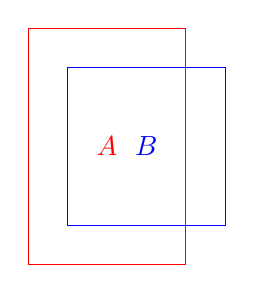
\begin{tikzpicture}
                    \draw[red] (0, 0) -- (2, 0) -- (2, 3) -- (0, 3) -- cycle;
                    \node[red] at (1, 1.5) {$A$};

                    \draw[blue] (0.5, 0.5) -- (2.5, 0.5) -- (2.5, 2.5) -- (0.5, 2.5) -- cycle;
                    \node[blue] at (1.5, 1.5) {$B$};
                \end{tikzpicture}
            \end{center}
            We consider the detection of the intersection over union (IoU) is above $0.5$;
            $$\text{IoU} = \frac{\red{A} \cap \blue{B}}{\red{A} \cup \blue{B}} > 0.5$$
            Another more complex piece of information we can extract is to perform \textbf{image segmentation}, allowing us to draw contours for each object.
            \subsubsection*{Applications}
                Computer vision is used in our lives daily;
                \begin{itemize}
                    \itemsep0em
                    \item \textbf{face detection}
                        \smallskip

                        This can be noticed in most camera applications on modern smartphones, when a small box is drawn around faces.
                        The algorithm first extracts \textbf{Haar} features from an image, and then determines (with these features) whether a region is a face or not.
                        \medskip

                        One example of these features is checking the contrast between the eyes and nose (horizontally); as the eyes tend to be quite dark in comparison.
                        Another contrast is checked, this time between your eyes, as the nose tends to be brighter.
                    \item \textbf{automatic number plate recognition}
                        \smallskip

                        Automated barriers in parking lots can read number plates in order to calculate how long a car stays.
                        Similarly, this can also be used to recognise building numbers, which is overlaid onto \textit{Google Maps}, allowing for a large database of street numbers to be built in an automated fashion.
                    \item \textbf{autonomous driving}
                    \item \textbf{image style transfer}
                        \smallskip

                        \textit{Choi et al. StarGAN: Unified Generative Adversarial Networks for Multi-Domain Image-to-Image Translation} - used for changing features on inputs.
                        Related to face motion capture (see \textit{Face2Face}).
                        Also see \textit{DeepFake}.
                    \item \textbf{Kinect}
                        \smallskip

                        Works by taking a depth image, segmenting it into body parts, locating key points and building a skeleton.
                    \item \textbf{design}
                        \smallskip

                        See \textit{OpenAI}'s \textit{DALL-E}, combining NLP and computer vision by generating images based on the concepts of words in a sentence.
                    \item \textbf{healthcare}
                        \smallskip

                        Medical image analysis can be used for disease diagnosis.
                        For example, identifying breast cancer lesions from mammograms.
                \end{itemize}
        \subsection*{Lecture 2 - Image Formation}
            An image, in RGB format, can be represented as pixels, each being three numbers.
            A digital image is formed from a lighting source being reflected into an optics sensor (eyes, cameras, etc).
            \subsubsection*{Light}
                A \textbf{point light source} originates from a single location in space, such as a small light bulb, or the sun.
                This can be described with three properties; location, intensity, and the spectrum.
                \medskip

                On the other hand, an \textbf{area light source} is more complex.
                For example, this could be a ceiling light; a rectangle of point lights.
            \subsubsection*{Reflectance}
                When light emitted from the source hits the surface of an object, it will be reflected.
                To describe this, we typically use the \textbf{bidirectional reflectance distribution function (BDRF)} to model this behaviour (where $\lambda$ is the wavelength, $L_r$ is the output power, and $E_i$ is the input power);
                $$f_r(\underbrace{\theta_i, \varphi_i}_\text{incident}, \underbrace{\theta_r, \varphi_r}_\text{reflected}, \lambda) = \dif{L_r}{E_i}$$
                While this is a very general model, it is very complex.
                \medskip

                As such, we can use \textbf{diffuse reflection}, where light is assumed to be scattered uniformly in all directions.
                This has a constant BRDF - this says that regardless of the incident or reflected directions, nor the wavelength, the power will be constant;
                $$f_r(\theta_i, \varphi_i, \theta_r, \varphi_r,, \lambda) = f_r(\lambda)$$
                \begin{center}
                    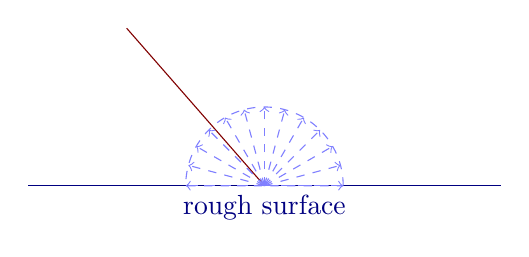
\begin{tikzpicture}
                        \draw[blue!50!black] (0, 0) edge[below] node{rough surface} (6, 0);
                        \draw[red!50!black] (1.25, 2) edge[->] (3, 0);
                        \draw[dashed, blue!50]
                        (4, 0) arc(0:180:1) -- cycle
                        (3, 0) edge[->] +(0:1)
                        (3, 0) edge[->] +(15:1)
                        (3, 0) edge[->] +(30:1)
                        (3, 0) edge[->] +(45:1)
                        (3, 0) edge[->] +(60:1)
                        (3, 0) edge[->] +(75:1)
                        (3, 0) edge[->] +(90:1)
                        (3, 0) edge[->] +(105:1)
                        (3, 0) edge[->] +(120:1)
                        (3, 0) edge[->] +(135:1)
                        (3, 0) edge[->] +(150:1)
                        (3, 0) edge[->] +(165:1)
                        (3, 0) edge[->] +(180:1);
                    \end{tikzpicture}
                \end{center}
                On the other hand, we can use \textbf{specular reflection} which performs reflections in a mirror-like fashion.
                The reflection and incident directions are symmetric with respect to the surface normal $\vec{n}$, such that $\theta_r = \theta_i$, with the same amount of power;
                \begin{center}
                    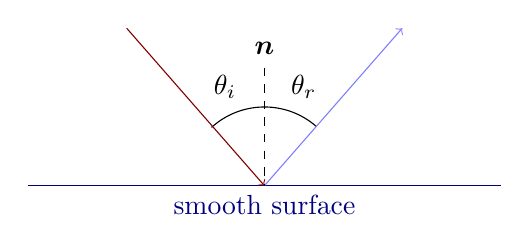
\begin{tikzpicture}
                        \draw (3, 0) ++(48.8:1) arc (48.8:132.2:1);
                        \draw[blue!50!black] (0, 0) edge[below] node{smooth surface} (6, 0);
                        \draw[red!50!black] (1.25, 2) edge[->] (3, 0);
                        \draw[blue!50] (4.75, 2) edge[<-] (3, 0);
                        \draw[dashed] (3, 1.5) -- (3, 0);

                        \node at (3, 1.75) {$\vec{n}$};
                        \node at (2.5, 1.25) {$\theta_i$};
                        \node at (3.5, 1.25) {$\theta_r$};
                    \end{tikzpicture}
                \end{center}
                While these two are the \textbf{ideal} cases, the majority of cases, we see a combination of both of those, as well as \textbf{ambient} illumination.
                Ambient illumination accounts for general illumination which could be complicated to model.
                For example, these could be repeated reflections between walls (which would be very difficult to calculate), and we instead assume that there is some light that exists in the 3D space representing the room.
                Another example could be a distance source, such as the sky (which has atmosphere).
                \medskip

                Combining these, we can use the \textbf{Phong} reflection model.
                This is an empirical model that describes how a surface reflects light as a combination of ambient, diffuse, and specular components.
            \subsubsection*{`Duality' with Computer Graphics}
                Using the game engine to produce example images is useful, as we are able to directly obtain the labels of objects from the engine itself, as well as visual output.
                As such, we can use these images as training for a model, since we also have an associated label map.
                This synthetic data is complementary to time-consuming manual annotations.
            \subsubsection*{Optics and Sensors}
                Both our eyes and cameras work in similar ways, with a lens governed by the thin lens equation, where $f$ denotes the focal length of the lens, $u$ denotes the distance from the subject to the lens, and $v$ denotes the distance from the lens to the image;
                $$\frac{1}{f} = \frac{1}{u} + \frac{1}{v}$$
                Our eyes work by light rays being focused by the cornea and lens onto the retina, where vision begins with two neural cells.
                The \textbf{cone} cells are responsible for colour vision, and function in bright light.
                On the other hand, the \textbf{rod} cells have little role in colour vision, but function in dim light.
                \medskip

                Humans have three types of cone cells (\textbf{trichromatic vision}), which have different response curves.
                The short cone cells respond to short wavelength lights (\violet{violet}, \blue{blue}), whereas the medium cone cells respond to medium wavelength lights (\textcolor{green}{green}), and long cone cells respond to long wavelength lights (\red{red}).
                Occasionally, there may be two cone cells, or four, which are referred to as \textbf{dichromacy} or \textbf{tetrachromacy} respectively.
                \medskip

                Note that colours are not objective physical properties of light or electromagnetic wave (which have a physical property of wavelength).
                Colour is a subjective feature, dependent on the visual perception of the observer.
                Since \textbf{rod} cells are more sensitive to light, they are the primary source of visual information at night.
                \medskip

                On the other hand, camera sensors have two common types;
                \begin{itemize}
                    \itemsep0em
                    \item \textbf{CCD} (charged-coupled device) \hfill often used in handheld cameras
                    \item \textbf{CMOS} (complementary metal-oxide semiconductor) \hfill used by most smartphone cameras
                \end{itemize}
                These sensors convert incoming light into electron charges, which are then read.
                \textbf{Bayer} filter arrays are a way to arrange RGB filters on sensors, half of which are green, and the remaining two quarters are red and blue.
                This mimics the human eyes, which are most sensitive to green light;
                \begin{center}
                    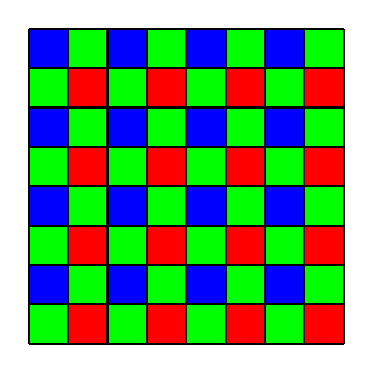
\begin{tikzpicture}[x=0.5cm, y=-0.5cm] % I should've just taken a screenshot, why do I keep doing this to myself
                        \foreach \i in {0,...,7} {
                            \foreach[evaluate={
                                \g=int(mod(\i + \j, 2);
                                \jm=int(mod(\j, 2))
                            }] \j in {0,...,7} {
                                \ifthenelse{\g = 1}
                                    {\def\col{green}}
                                    {\ifthenelse{\jm = 0}
                                        {\def\col{blue}}
                                        {\def\col{red}}}
                                \draw[fill=\col, draw=none] (\i, \j) -- (\i + 1, \j) -- (\i + 1, \j + 1) -- (\i, \j + 1) -- cycle;
                            }
                        }
                        \foreach \x in {0,...,8} {\draw[thick] (\x, 0) -- (\x, 8);}
                        \foreach \y in {0,...,8} {\draw[thick] (0, \y) -- (8, \y);}
                    \end{tikzpicture}
                \end{center}
                CMOS works by having sensors underneath each of these filtered portions, which can report an electrical signal.
                However, note that only one colour is available at each pixel (therefore the rest must be interpolated from the neighbours, by using bilinear interpolation; which simply averages the 4 neighbours).
                For example, consider the following pixel (denoted as a white cross);
                \begin{center}
                    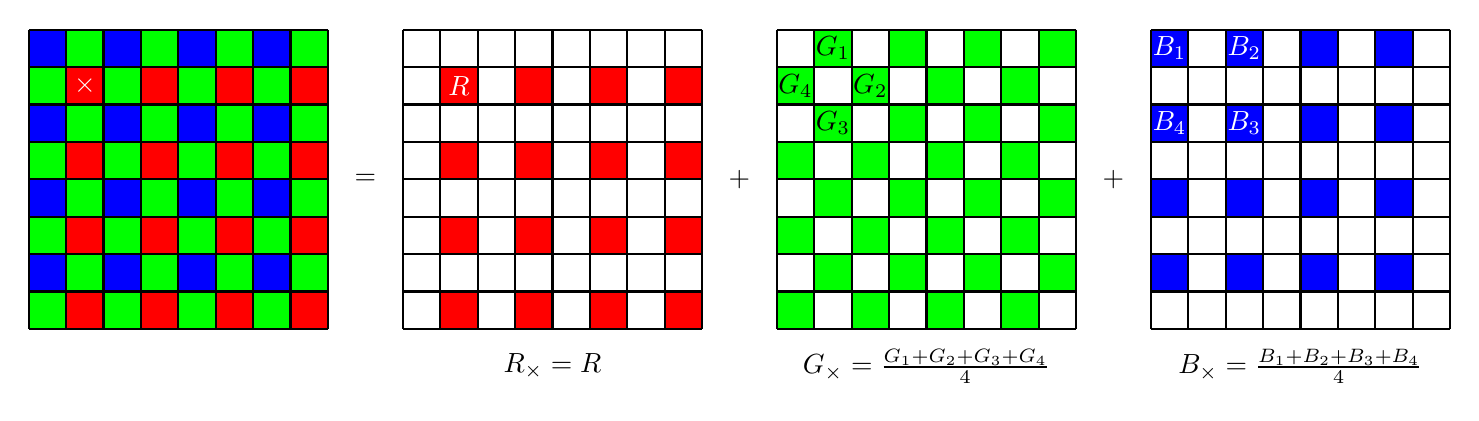
\begin{tikzpicture}[x=0.475cm, y=-0.475cm] % I should've just taken a screenshot, why do I keep doing this to myself
                        \begin{scope}[shift={(0, 0)}]
                            \foreach \i in {0,...,7} {
                                \foreach[evaluate={
                                    \g=int(mod(\i + \j, 2);
                                    \jm=int(mod(\j, 2))
                                }] \j in {0,...,7} {
                                    \ifthenelse{\g = 1}
                                        {\def\col{green}}
                                        {\ifthenelse{\jm = 0}
                                            {\def\col{blue}}
                                            {\def\col{red}}}
                                    \draw[fill=\col, draw=none] (\i, \j) -- (\i + 1, \j) -- (\i + 1, \j + 1) -- (\i, \j + 1) -- cycle;
                                }
                            }
                            \foreach \x in {0,...,8} {\draw[thick] (\x, 0) -- (\x, 8);}
                            \foreach \y in {0,...,8} {\draw[thick] (0, \y) -- (8, \y);}

                            \node[white] at (1.5, 1.5) {$\times$};
                        \end{scope}
                        \begin{scope}[shift={(10, 0)}]
                            \foreach \i in {0,...,7} {
                                \foreach[evaluate={
                                    \g=int(mod(\i + \j, 2);
                                    \jm=int(mod(\j, 2))
                                }] \j in {0,...,7} {
                                    \ifthenelse{\g = 1}
                                        {\def\col{white}}
                                        {\ifthenelse{\jm = 0}
                                            {\def\col{white}}
                                            {\def\col{red}}}
                                    \draw[fill=\col, draw=none] (\i, \j) -- (\i + 1, \j) -- (\i + 1, \j + 1) -- (\i, \j + 1) -- cycle;
                                }
                            }
                            \foreach \x in {0,...,8} {\draw[thick] (\x, 0) -- (\x, 8);}
                            \foreach \y in {0,...,8} {\draw[thick] (0, \y) -- (8, \y);}

                            \node[white] at (1.5, 1.5) {$R$};
                        \end{scope}
                        \begin{scope}[shift={(20, 0)}]
                            \foreach \i in {0,...,7} {
                                \foreach[evaluate={\g=int(mod(\i + \j, 2)}] \j in {0,...,7} {
                                    \ifthenelse{\g = 1}
                                        {\def\col{green}}
                                        {\def\col{white}}
                                    \draw[fill=\col, draw=none] (\i, \j) -- (\i + 1, \j) -- (\i + 1, \j + 1) -- (\i, \j + 1) -- cycle;
                                }
                            }
                            \foreach \x in {0,...,8} {\draw[thick] (\x, 0) -- (\x, 8);}
                            \foreach \y in {0,...,8} {\draw[thick] (0, \y) -- (8, \y);}

                            \node at (1.5, 0.5) {$G_1$};
                            \node at (2.5, 1.5) {$G_2$};
                            \node at (1.5, 2.5) {$G_3$};
                            \node at (0.5, 1.5) {$G_4$};
                        \end{scope}
                        \begin{scope}[shift={(30, 0)}]
                            \foreach \i in {0,...,7} {
                                \foreach[evaluate={
                                    \g=int(mod(\i + \j, 2);
                                    \jm=int(mod(\j, 2))
                                }] \j in {0,...,7} {
                                    \ifthenelse{\g = 1}
                                        {\def\col{white}}
                                        {\ifthenelse{\jm = 0}
                                            {\def\col{blue}}
                                            {\def\col{white}}}
                                    \draw[fill=\col, draw=none] (\i, \j) -- (\i + 1, \j) -- (\i + 1, \j + 1) -- (\i, \j + 1) -- cycle;
                                }
                            }
                            \foreach \x in {0,...,8} {\draw[thick] (\x, 0) -- (\x, 8);}
                            \foreach \y in {0,...,8} {\draw[thick] (0, \y) -- (8, \y);}

                            \node[white] at (0.5, 0.5) {$B_1$};
                            \node[white] at (2.5, 0.5) {$B_2$};
                            \node[white] at (2.5, 2.5) {$B_3$};
                            \node[white] at (0.5, 2.5) {$B_4$};
                        \end{scope}
                        \node at (9, 4) {$=$};
                        \node at (19, 4) {$+$};
                        \node at (29, 4) {$+$};

                        \node at (14, 9) {$R_\times = R$};
                        \node at (24, 9) {$G_\times = \frac{G_1 + G_2 + G_3 + G_4}{4}$};
                        \node at (34, 9) {$B_\times = \frac{B_1 + B_2 + B_3 + B_4}{4}$};
                    \end{tikzpicture}
                \end{center}
                Note that the use of different filters, and this interpolation, can lead to slightly different colours between cameras.
            \subsubsection*{Image Representation}
                The earliest colour space was described in 1931 by CIE, by performing a colour matching experiment.
                In this experiment, an observer attempts to match different levels of red, green, and blue lights to match a target light.
                This allows for colours to be represented in 3D space, as $(X, Y, Z)$, corresponding to the different levels.
                Colours can also be represented on a 2D plane, by normalising brightness;
                \begin{align*}
                    x & = \frac{X}{X + Y + Z} \\
                    y & = \frac{Y}{X + Y + Z} \\
                    z & = \frac{Z}{X + Y + Z} \\
                    & = 1 - x - y & \text{therefore redundant}
                \end{align*}
                Here $X, Y, Z$ are primary colours ($R, G, B$), and $x, y$ are chromacity / colour after removing brightness.
                This is much easier to draw.
                However, this colour space, also known as the \textbf{gamut} of human vision, was invented before computer screens.
                \medskip

                The sRGB (standard RGB) space was created by \textit{HP} and \textit{Microsoft} in 1996 for use on monitors, printers, and the internet.
                \begin{center}
                    \begin{tabular}{lcc}
                        sRGB definition & $x$ & $y$ \\
                        \hline
                        \red{red} & 0.64 & 0.33 \\
                        \textcolor{green}{green} & 0.30 & 0.60 \\
                        \blue{blue} & 0.15 & 0.06
                    \end{tabular}
                \end{center}
                This is represented by a triangle (which is a subset) in the gamut of human vision.
                As this is a subset, it cannot produce all the colours visible by the human eye.
                \medskip

                There are other colour spaces, such as HSV, CMYK, and so on.
                Note that CMYK is a \textbf{subtractive} colour model, starting from white, whereas RGB is an \textbf{additive} colour model, where we start from black.
                There can also be an alpha channel in RGB, which represents transparency.
                In a greyscale image, the three components are equal, hence only require one number.
            \subsubsection*{Quantisation}
                Note that this is covered in lecture 3.
                \medskip

                \textbf{Quantisation} maps a continuous signal to a discrete signal.
                The pictures from a camera are a continuous signal, but when it is stored on the camera, it is quantised to a discrete signal.
                Numerical errors can occur during this process, and the magnitude of the errors depends on the number of bits used (less error with more bits; 16 bits can store from 0 to 65535, compared to 8 bits storing from 0 to 255).
                \medskip

                Physically, an analog-to-digital convert (ADC) is used to perform the conversion.
                The energy of photons are converted into voltage, amplified, and then converted.
            \subsubsection*{Compression}
                In order to reduce the cost of storage to transmission, compression may be used.
                Lossy compression loses information after the compression (such as discrete cosine transform (DCT) in JPEG, often used for images or videos).
                However, lossless compression can also reduce the file size (less efficient compared to lossy), and is preferred for archival purposes or important imaging, where detail needs to be recovered.
        \subsection*{Lecture 3 - Image Filtering}
            Note that in this course, most of the examples will be done on greyscale images, but can be applied to the channels individually.
            Some examples of filters include;
            \begin{itemize}
                \itemsep0em
                \item identity filter
                    \smallskip

                    Does nothing to the image.
                \item low-pass / smoothing (moving average, Gaussian)
                    \smallskip

                    Removes high-frequency signals, and keep low-frequency signals.
                \item high-pass / sharpening
                    \smallskip

                    Similar to the previous filter (keeps high-frequency signals, and removes low-frequency).
                \item denoise (median, non-local means, block-matching and 3D filtering)
            \end{itemize}
            \subsubsection*{Moving Average Filter}
                This is commonly used for 1D signal processing (time series), such as stocks, which can be quite noisy.
                To smooth out a noisy curve, it moves a window across the signal (and calculates the average value within the window) - the larger the window size, the smoother the result.
                \medskip

                In a two dimensional case, we can use a \textbf{filter kernel} (for example, with a $3 \times 3$ kernel);
                $$\frac{1}{9} \begin{bmatrix}
                    1 & 1 & 1 \\
                    1 & 1 & 1 \\
                    1 & 1 & 1
                \end{bmatrix}$$
                At each pixel, we apply the kernel centred at the pixel, and take the average of the pixels around it (and itself) to create a new output image.
                When we blur with a larger kernel, such as $7 \times 7$, we end up with a blurrier image.
                Note that the output image is smaller than the input image.
                We can pad the image with zeroes (anything outside of the picture is 0), or by mirroring the pixels (copying the boundary pixels).
                \medskip

                Consider an image of size $N \times N$, and a kernel size of $K \times K$.
                At each pixel, we perform $K^2$ multiplications (by the kernel weights), and then $K^2 - 1$ summations.
                This has to be done for each pixel, hence $N^2$ times.
                Therefore this results in $N^2 K^2$ multiplications and $N^2 (K^2 - 1)$ summations; giving a \textbf{complexity} of $O(N^2 K^2)$.
                However, we'd like to reduce this, if possible.
                \medskip

                If a big filter can be separated as two filters (\textbf{separable filter}) applied consecutively, we can perform the first operation, and then the second.
                An average in a 2D window can be done as an average across rows (horizontal), and then an average across columns (vertical);
                $$\begin{bmatrix}
                    \frac{1}{9} & \frac{1}{9} & \frac{1}{9} \\
                    \frac{1}{9} & \frac{1}{9} & \frac{1}{9} \\
                    \frac{1}{9} & \frac{1}{9} & \frac{1}{9}
                \end{bmatrix} = \begin{bmatrix}
                    \frac{1}{3} & \frac{1}{3} & \frac{1}{3}
                \end{bmatrix} * \begin{bmatrix}
                    \frac{1}{3} \\ \frac{1}{3} \\ \frac{1}{3}
                \end{bmatrix}$$
                Doing these two filters, we end up with an equivalent result to the original 2D filter.
                Note that $*$ is a convolution (see next lecture).
                \medskip

                Consider the complexity of separable filtering.
                The image size remains as $N \times N$, however we have two kernels, of $1 \times K$ and $K \times 1$ respectively.
                At each pixel we do $K$ multiplications followed by $K - 1$ summations.
                Again, this is done for $N^2$ pixels, and twice (once for each filter).
                Therefore, the total number of multiplications is $2N^2K$ multiplications and $2N^2(K - 1)$ summations.
                This is better, in contrast to the original complexity, as we have complexity of $O(N^2K)$ - which will make a difference for large $K$.
                \medskip

                A moving average filter removes high frequency signals (noise or sharpness), which results in a smooth but blurry image.
            \subsubsection*{Gaussian Filter}
                The kernel is a 2D Gaussian distribution;
                $$h(i, j) = \frac{1}{2 \pi \sigma^2} e^{-\frac{i^2 + j^2}{2 \sigma^2}}$$
                Here we have $i, j = 0, 0$ as the centre of the kernel.
                While the support is infinite, small values outside the range $[-k\sigma, k\sigma]$ can be ignored (very small values, such as $k=3$ or $k=4$).
                Note that $\sigma$ is a manually defined parameter.
                This is a separable filter, which is equivalent to two 1D Gaussian filters with the same $\sigma$, with one along the $x$-axis and the other along the $y$-axis;
                \begin{align*}
                    h(i, j) & = h_x(i) * h_y(j) \\
                    h_x(i) & = \frac{1}{\sqrt{2 \pi \sigma^2}} e^{-\frac{i^2}{2\sigma^2}}
                \end{align*}
            \subsubsection*{High-pass Filter}
                One design is to do the following;
                $$\underbrace{\begin{bmatrix}
                    0 & 0 & 0 \\
                    0 & 1 & 0 \\
                    0 & 0 & 0
                \end{bmatrix}}_\text{identity} + \underbrace{\left(\begin{bmatrix}
                    0 & 0 & 0 \\
                    0 & 1 & 0 \\
                    0 & 0 & 0
                \end{bmatrix} - \begin{bmatrix}
                    \frac{1}{9} & \frac{1}{9} & \frac{1}{9} \\
                    \frac{1}{9} & \frac{1}{9} & \frac{1}{9} \\
                    \frac{1}{9} & \frac{1}{9} & \frac{1}{9}
                \end{bmatrix}\right)}_\text{high-frequency} = \begin{bmatrix}
                    -\frac{1}{9} & -\frac{1}{9} & -\frac{1}{9} \\
                    -\frac{1}{9} & \frac{17}{9} & -\frac{1}{9} \\
                    -\frac{1}{9} & -\frac{1}{9} & -\frac{1}{9}
                \end{bmatrix}$$
                We can add a high frequency signal to the identity, in order to enhance it.
            \subsubsection*{Median Filter}
                This is a non-linear filter (not performing an average calculation by multiplication).
                This moves a sliding window, and replaces the centre pixel with the median value in the window - this is not a linear equation.

\end{document}